\section{Evaluation}
\label{sec:eval}

\subsection{Experimental setup}
\label{sec:eval-setup}

\noindent
We implemented {\sys} on {\verl}---the state-of-the-art
post-training framework that
has integrated known inference optimizations
including CUDA graph~\cite{vllm-code},
prefix caching~\cite{DBLP:journals/corr/abs-2402-03300} 
and FlashAttention kernels~\cite{DBLP:conf/nips/ShahBZTRD24}. 

\stitle{Testbed. \,} 
We evaluated {\sys} on a production training cluster
with up to 512\,GPUs.
These GPUs are organized into nodes where each node contains eight Hopper (80\,GB) GPUs
interconnected with {400}\,GB/s NVLink,
and inter-node GPUs have up to 400\,Gbps RDMA connections.

\stitle{Evaluated traces: model, algorithm and rollout temperature.} \,
Similar to prior works~\cite{dapo,hybridflow,streamrl}, 
we evaluated Qwen series models (\eg{Qwen2.5-32B})
as they are one of the most popular open-sourced LLMs~\cite{dapo,DBLP:journals/corr/abs-2504-05118,gspo}
and are commonly used by algorithm designers. 
We evaluated on {3} 
representative 200-step training traces based on production setups
with different (popular) post-training algorithms: \\[-18pt]

\begin{itemize}[leftmargin=*,leftmargin=10pt,itemindent=0pt]
    \itemsep0.5em
    \item \textbf{GRPO-32B-20K.} 
    This trace trains Qwen2.5-32B~\cite{qwen2.5}
    with the GRPO~\cite{DBLP:journals/corr/abs-2402-03300} algorithm,
    a representative value-model-free post-training method 
    that trains high-quality models like DeepSeek series~\cite{DBLP:journals/corr/abs-2509-02547,deepseek-r1}.
    The trace samples a total batch of 8,192 prompts at each step\footnote{\footnotesize{Including the group sampling factor. }},
    where for each batch, the model generates responses with a budget of 20\,K tokens.
    The trace runs on 256\,GPUs with a tensor parallelism (TP) degree of 4 for
    each rollout worker, so the initial per-worker batch size is 128.  \\[-18pt]

    \item \textbf{DAPO-32B-20K.} 
    This trace also trains Qwen2.5-32B using DAPO~\cite{dapo}---a
    trending algorithm in AI academy and industry~\cite{DBLP:journals/corr/abs-2508-03501,DBLP:journals/corr/abs-2505-23433}---with
    a per-step batch size of 16,384 and a response budget of 20\,K tokens.
    The trace runs on 256 GPUs with a 4-degree TP for each rollout worker,
    so the per-worker batch size is 256.
    DAPO requires a larger per-step batch size because its training
    method filters out low-quality responses generated during the rollout. \\[-18pt]

    \item \textbf{PPO-32B-20K.} 
    PPO is another widely used RL algorithm~\cite{DBLP:journals/corr/SchulmanWDRK17,DBLP:journals/corr/abs-2504-05118}.
    The trained model is Qwen2.5-32B, and the PPO trace is different in 
    (1) it utilizes another 32B critic model to generate value and trains the critic together with the actor model;
    (2) meanwhile, it samples only one response per prompt. The per-step batch size is 4,096 
    and the maximum response length is 20\,K tokens. 
    We run the trace on the same cluster setup like the above two traces. \\[-14pt]
\end{itemize}

\noindent
For all experiments, we set the sampling temperature of LLM generation
to 1.0---a common setup in post-training~\cite{deepseek-r1,DBLP:journals/corr/abs-2402-03300,DBLP:journals/corr/abs-2507-20534}---which, however, 
has a negative impact on speculative decoding
~\cite{DBLP:conf/acl/XiaYDW00L0S24,DBLP:journals/corr/abs-2509-04474,DBLP:journals/corr/abs-2510-26475}.
% as also confirmed by the \highlight{algorithm designers} at {\company}.
LLM post-training requires such settings to explore more diverse responses
and avoid entropy collapse~\cite{DBLP:journals/corr/abs-2505-23585,dapo,DBLP:journals/corr/abs-2504-05118};
otherwise, the trained model suffers from premature convergence, 
which limits its potential for further performance gains.
% the trained model will generate similar results for
% the same prompt where the similarity includes
% both the output length and the content.

Due to GPU time constraints, our experiments focus on dense 32\,B
models, but we have also conducted experiments on a large 
Qwen3-235B MoE model~\cite{qwen3}
in \textsection{\ref{sec:eval-moe}} to demonstrate the effectiveness of {\sys}. 
%The MoE rollout requires an up to {5.1}\,$\times$ longer time. 

\stitle{Evaluating metrics. \,}
We focus on reporting the end-to-end training time and the rollout time---since
training time is the most critical metric for algorithm developers
and rollout dominates the time in \textsection{\ref{sec:bg-post-training}}.
To ensure representative evaluation, we uniformly sample at least 10\% of all training steps,
using the trained checkpoints at the sampled steps for generation,
and report their training and rollout time.

\stitle{Baselines. \,}
We compared {\sys} with the following baselines and carefully tuned their
implementations and performance.
All systems rollout with vLLM v0.10.0 engine~\cite{vllm-code}.
Specifically,
the decoding latency of Qwen2.5-32B model
is lower to 13\,ms when per-worker batch size is 1 on our platform. 
%Notice that we set sampling temperature to 1.0 (high token diversity) following common 
%production post-training practice.
For all baselines, we report the optimal configuration for training,
% preparation and learning phases,
i.e., an FSDP degree of 32 and 8-way sequence parallelism~\cite{ulysses-sp}.
\\[-10pt]

\begin{itemize}[leftmargin=*,leftmargin=10pt,itemindent=0pt]
    \itemsep0.5em
    \item \textbf{\verl~\cite{DBLP:conf/eurosys/ShengZYWZZPL025}}
    is an open-sourced post-training system used by {\company}
    and {\sys} is based on it.
    Besides the inference optimizations mentioned in the beginning of the section,
    it further incorporates techniques like efficient parameter
    to quickly update parameters for the rollout. \\[-10pt]

    \item \textbf{RLHFuse~\cite{rlhfuse}} 
    is the state-of-the-art post-training system that overlaps
    the prepare and rollout phases to reduce bubbles caused by
    long-tailed generation.
    Since it is not open-sourced, we carefully re-implemented its design
    and achieve a similar speedup on short-context tasks. 
    \\[-18pt]

    \item \textbf{{\verl} (2\,$\times$)} 
    provisions 2\,$\times$ of GPUs used by the original trace for {\verl}, 
    which serves as the optimal performance of using more GPUs 
    to accelerate RL like RLBoost~\cite{rlboost}.  \\[-18pt]

    \item \textbf{{\verl} + (vanilla) model-spec.}
    To illustrate the effectiveness of our proposed techniques,
    we also compare {\verl} by incorporating model-based speculative
    decoding in inference systems~\cite{spd,specinfer}.
    We run coupled speculation described in \textsection{\ref{sec:overview}}.
    The draft method is selected based on the first phase of our Fastest-of-N speculation.
    For 32B training, we found 0.5B is a sweet point to accelerate. \\[-18pt]

    \item \textbf{{\verl} + (vanilla) n-gram.}
    % N-gram is a category of training-free draft methods. It employs a dynamic token cache
    % to retrieve redundant sequences from recent outputs~\cite{pld,lookahead,DBLP:conf/acl/HuWZZLCZ25}.
    % We carefully enhance vLLM's n-gram to match the implementation of the {\sota} works~\cite{DBLP:conf/acl/HuWZZLCZ25,rhymerl} 
    % as a speculative decoding baseline,
    % to compare its effectiveness with our approach.
    N-gram is a popular speclative decoding method used by other works~\cite{rhymerl,seer}
    to accelerate rollout. 
    We have integrated a baseline of it using vLLM's n-gram (v0.10.0), 
    with enhancement of recent techniques like SAM~\cite{DBLP:conf/acl/HuWZZLCZ25} 
    to match their implementation as much as possible (since their code is not open-sourced). \\[-18pt]

    \iffalse    
    We also enhance {\verl} with vanilla speculative decoding~\cite{spd}.
    {Specifically, we use small-LLM-based speculation to let readers better understand how our design improve existing speculative decoding methods.}
    We carefully port it on vllm to benefit from its v1 codebase.
    \fi

    % \item \textbf{EAGLE-as-draft.}
    % \item \textbf{Lookahead-as-draft.}

\end{itemize}

\stitle{Draft methods used by {\sys}. \,}
Unless otherwise specified, 
we select the available drafters for Qwen2.5-32B 
% after the pre-training pipeline
before the post-training pipeline:
Qwen2.5-0.5B~\cite{qwen2.5}, Qwen2.5-1.5B---as well as an n-gram drafter~\cite{vllm-code,DBLP:conf/acl/HuWZZLCZ25}.
Other drafting methods, such as EAGLE~\cite{eagle,eagle-2,eagle-3}, 
require additional training support,
which is not supported by all our evaluated models. 

%{\sys} works well on all temperature setups.

\subsection{End-to-end post-training performance}
\label{sec:eval-e2e}

\begin{figure}[!t]
    %    \vspace{2mm}
        \begin{minipage}{1\linewidth}
        \hspace{-1mm}
        \centering    
        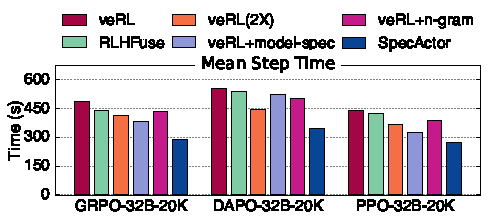
\includegraphics[width=\columnwidth]{data/e2e-throughput.pdf} \\[1pt]    
        \end{minipage} \\[0pt]
        \begin{minipage}{1\linewidth}
        \caption{\small{%
        {
            The mean training step time
            of {\sys} running different training traces
            with different approaches. 
        }}}
        \label{fig:e2e}
        \end{minipage} \\[-15pt]
\end{figure}

\begin{figure}[!t]
    %    \vspace{2mm}
        \begin{minipage}{1\linewidth}
        \hspace{-1mm}
        \centering    
        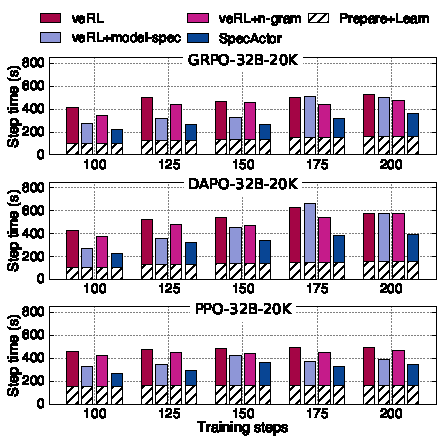
\includegraphics[width=\columnwidth]{data/e2e-multi-step.pdf} \\[1pt]    
        \end{minipage} \\[1pt]
        \begin{minipage}{1\linewidth}
        \caption{\small{%
        {
        A breakdown of post-training process of different approaches on
        different training traces.
        }}}
        \label{fig:breakdown}
        \end{minipage} \\[-15pt]
\end{figure}

\noindent
\fig{fig:e2e} presents the end-to-end training step time of different approaches
on the traces. 
We measure all 1/10 of the sampled training steps and report the mean step time of 
different approaches. 
Note that each step uses the exact same model checkpoint and prompt batch 
in the trace to faithfully reproduce the real-world workloads. 
{\sys} achieves {1.5--1.7\,$\times$} faster end-to-end 
training compared to baselines like veRL and RLHFuse.
For vanilla speculative decoding baselines, 
{\sys} achieves {1.2--1.5\,$\times$} shorter training time in different traces.
Even compared with {\verl} (2\,$\times$) that uses twice the GPUs, 
{\sys} still achieves {1.3--1.4\,$\times$} training speedup.
The key contributor is the acceleration of rollout via our
efficient mechanisms: 
for the rollout phase, {\sys} achieves {2.0--2.4}\,$\times$ faster 
mean generation speed than {\verl}.

Notably, {\sys} achieves up to {1.4--2.0\,$\times$} shorter average rollout time 
even compared with methods that also incorporate speculative decoding acceleration,
\ie{model-spec and n-gram}.
This is because:
First, both of them suffer from inefficiency due to large per-worker batch size
in the initial phase.
% The batch size decreases ratio during the first half of the rollout is 
% \TODO{xx,xx and xx}, respectively. 
Second, both of them, especially n-gram, have low acceptance rates for the straggler requests,
because the n-gram method performs poorly in high temperature sampling
with few history prompts commonly found in training traces.
Specifically, the skipped iteration of the last finished requests of n-gram 
is {16.9--43.6}\,\% across the traces,
{while {\sys} achieves 40.9--73.5\,\%
thanks to our Fastest-of-N speculation.}


\begin{figure}[!t]
       \vspace{2mm}
        \begin{minipage}{1\linewidth}
        \hspace{-1mm}
        \centering    
        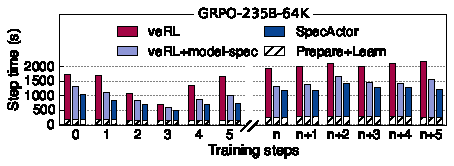
\includegraphics[width=\columnwidth]{data/e2e-moe.pdf} \\[1pt]    
        \end{minipage} \\[1pt]
        \begin{minipage}{1\linewidth}
        \caption{\small{%
        {
        A breakdown of post-training steps of Qwen3-235B.
        }}}
        \label{fig:moe}
        \end{minipage} \\[-15pt]
\end{figure}

\subsection{Performance on large MoE models}
\label{sec:eval-moe}

\noindent
\fig{fig:moe} presents the performance of {\sys}
when training a Qwen3-235B MoE model~\cite{qwen3} on 256\,GPUs
with GRPO algorithm.
Due to limited GPU time and the availability of checkpoints,
we only evaluated a few steps:
0--5 at the start of the post-training (using the Qwen3-235B-Instruct-2507)
and $n, \ldots, n+5$ from the end of the training (using the Qwen3-235B-Thinking-2507).
The difference is that the later steps tend to generate longer responses.
The per-step batch size is 256---a slightly smaller batch size due to
limited GPU memory, and each rollout worker uses expert parallelism (EP) of 8
for high decode efficiency.

{We expand the draft ladder with small models produced before
post-training pipeline~\cite{qwen3}: Qwen3-4B-2507-Instruct 
(released together with 235B), Qwen3-0.6B and Qwen3-1.7B.}

{\sys} improves the training time by {1.4--2.3}\,$\times$,
with {1.5--2.6}\,$\times$ rollout acceleration compared to {\verl}.
It also outperforms vanilla mode-spec by {1.1--1.5}\,$\times$, 
thanks to our decoupled and Fastest-of-N speculation.
Notice that even with a relatively small per-step batch size,
verification overhead is still high in MoE models as it is exacerbated
by expert communication~\cite{DBLP:journals/corr/abs-2505-19645}. 
{We also found that 
Qwen3-4B-2507-Instruct performs significantly better in speculation 
than the other two, we suspect its training pipeline is closely coupled
with 235B and thus has better alignment with it.}
% Our Fastest-of-N speculation also effectively improves the acceptance rates

\subsection{Performance across different steps}
\label{sec:eval-breakdown}

\noindent
%As the prompts and model checkpoints evolve in post-training, 
As the trained model evolves across different training steps,
the effectiveness of speculative decoding varies.
Thus, we further present the detailed latency breakdown of different
training steps in \fig{fig:breakdown}.
For ease of presentation, we selectively
present part of the training steps between {100--200} training steps to examine speculative decoding's effect
in real-world post-training.
The gap is sufficiently large as confirmed by internal accuracy tests,
so the "smartness" of the trained models in different sampling
steps varies.

First we can see that 
{\sys} still achieves the shortest rollout time in all steps.
Specifically, at $175^{th}$ and $200^{th}$ steps, 
veRL + model-spec and n-gram 
fail to provide acceleration because 
as models becomes smarter, they tend to produce longer responses~\cite{deepseek-r1} for more prompts,
leading to more rollout steps under a relatively large per-worker batch size.
In contrast, {\sys} consistently reduces rollout time by {1.8--2.7}\,$\times$,
and is faster than vanilla speculative decoding baselines by 
{1.4--2.6}\,$\times$, {1.2--2.2}\,$\times$, {1.2--2.6}\,$\times$ in different training traces.
Thanks to the quick generation,
more workers finish at early time,
leaving {\sys} sufficient room for FoN scheduling. 

\subsection{Ablation study}

\begin{figure}[!t]
    %    \vspace{2mm}
        \begin{minipage}{1\linewidth}
        \hspace{-1mm}
        \centering    
        
\includegraphics[width=\columnwidth]{data/ablation.pdf} \\[1pt]    
        \end{minipage} \\[0pt]
        \begin{minipage}{1\linewidth}
        \caption{\small{%
        {            
            Ablation study of using the DAPO-32B-20K trace.
            The other trace shows similar results.
        }}}
        \label{fig:ablation}
        \end{minipage} \\[-15pt]
\end{figure}

%\nospacestitle{Effectiveness of our techniques. \,}
\noindent
\fig{fig:ablation} conducts an ablation study to
examine the effectiveness of different proposed techniques described in \textsection{\ref{sec:design}}.
We reported only one step here due to space limitation, and other steps in different traces 
show similar results.

First, we can see that vanilla speculative decoding reduces only {2.6\,\%} rollout end-to-end latency,
which is small due to the inefficiency of large-batch verification 
and suboptimal draft method for the tailed requests. 

Thanks to our decoupled speculative decoding,
we accelerate rollout by {1.3\,$\times$}.
Based on decoupled speculative decoding,
our dynamic reconfiguration
further shortens the rollout time by {1.2\,$\times$} thanks
to a better initial execution configuration and dynamic reconfiguration
of workers with low acceptance rates to reduce wasted tokens.
Finally, our Fastest-of-N speculative decoding further accelerates end-to-end rollout
by {1.2\,$\times$}, thanks to its ability to leverage multiple draft methods
to improve acceptance rates for straggler requests.


\begin{figure}[!t]
    %    \vspace{2mm}
        \begin{minipage}{1\linewidth}
        \hspace{-1mm}
        \centering    
        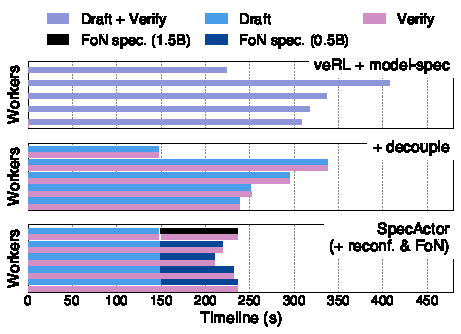
\includegraphics[width=\columnwidth]{data/timeline.pdf} \\[1pt]    
        \end{minipage} \\[1pt]
        \begin{minipage}{1\linewidth}
        \caption{\small{%
        {
    An in-depth analysis of the execution of different approaches on
    the {$200^{th}$}  step of DAPO-32B-20K trace. 
    We sample workers that contains the tailed requests for ease of presentation.
        }}}
        \label{fig:timeline}
        \end{minipage} \\[-5pt]
\end{figure}

\subsection{An in-depth look at {\sys} in action}
\label{sec:eval-timeline}

\noindent
We conclude our evaluation of {\sys} by presenting an in-depth analysis
of the work done by different workers during the rollout with our techniques in
\fig{fig:timeline}.
%shows the execution timeline of the selected training step.
To ease presentation, we only sampled {5} workers,
with a deliberate focus on the worker that finish early
and the slowest four workers.

First, from the first row of \fig{fig:timeline}
we can see that vanilla speculative decoding still
suffers from long-tailed workers
because during the initial phase all workers execute slower
and at the end the initially selected draft method
cannot accelerate the slowest requests.
With decoupled speculative decoding (the second row), we improve speculative decoding performance
by {1.1--1.5}\,$\times$ but still suffer from long-tailed requests
due to suboptimal draft method.
With Fastest-of-N speculative decoding activated, the freed workers are assigned
different draft methods (we use different color blocks to indicate different draft methods)
at 151s in \fig{fig:timeline}.
This subsequently accelerates the slowest requests by {1.5}\,$\times$.

